\chapter{p3 = 6 (4 graphs)}
\newpage\begin{figure}
  \begin{tikzpicture}
      \draw
        (0.0:2) node (0){0}
        (72.0:2) node (1){1}
        (144.0:2) node (2){2}
        (216.0:2) node (3){3}
        (288.0:2) node (4){4};
      \begin{scope}[-]
        \draw (0) to (4);
        \draw (1) to (4);
        \draw (2) to (4);
        \draw (3) to (4);
      \end{scope}
    \end{tikzpicture}
\end{figure}
\begin{itemize}
\item signature: 0001001011
\item g: Graph with 5 nodes and 4 edges
\item order: 5
\item size: 4
\item max degree: 4
\item degrees: 1,1,1,1,4
\item is tree: 1
\item is bipartite: 1
\item has bridge: 1
\item is chordal: 1
\item is complete: 0
\item min cycle basis weight: 0
\item min cycle basis size: 0
\item diameter: 2
\item radius: 1
\item is eulerian: 0
\item is planar: 1
\item number of faces: 1
\item is regular: 0
\item p3: 6
\item p4: None
\item property hash: 5d3cee38766e85d6aae60827273f46765c56c2e419981b8cc80fde98fe1dcf67
\end{itemize}
\newpage
\begin{figure}
  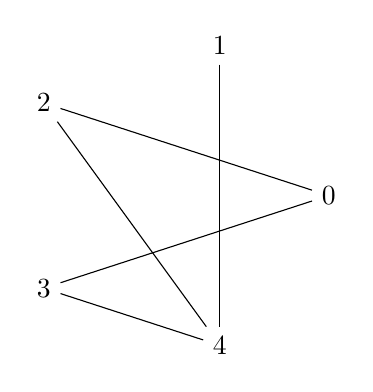
\begin{tikzpicture}
      \draw
        (0.0:2) node (0){0}
        (72.0:2) node (1){1}
        (144.0:2) node (2){2}
        (216.0:2) node (3){3}
        (288.0:2) node (4){4};
      \begin{scope}[-]
        \draw (0) to (2);
        \draw (0) to (3);
        \draw (1) to (4);
        \draw (2) to (4);
        \draw (3) to (4);
      \end{scope}
    \end{tikzpicture}
\end{figure}
\begin{itemize}
\item signature: 0110001011
\item g: Graph with 5 nodes and 5 edges
\item order: 5
\item size: 5
\item max degree: 3
\item degrees: 1,2,2,2,3
\item is tree: 0
\item is bipartite: 1
\item has bridge: 1
\item is chordal: 0
\item is complete: 0
\item min cycle basis weight: 4
\item min cycle basis size: 1
\item diameter: 3
\item radius: 2
\item is eulerian: 0
\item is planar: 1
\item number of faces: 2
\item is regular: 0
\item p3: 6
\item p4: 2
\item property hash: 02d3b8854a44375b83125826e105748a8e5daa0fee328587d5b3929392c8697c
\end{itemize}
\newpage
\begin{figure}
  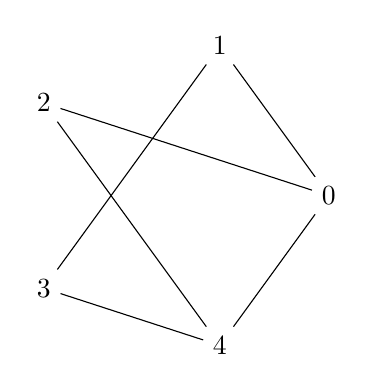
\begin{tikzpicture}
      \draw
        (0.0:2) node (0){0}
        (72.0:2) node (1){1}
        (144.0:2) node (2){2}
        (216.0:2) node (3){3}
        (288.0:2) node (4){4};
      \begin{scope}[-]
        \draw (0) to (1);
        \draw (0) to (2);
        \draw (0) to (4);
        \draw (1) to (3);
        \draw (2) to (4);
        \draw (3) to (4);
      \end{scope}
    \end{tikzpicture}
\end{figure}
\begin{itemize}
\item signature: 1101010011
\item g: Graph with 5 nodes and 6 edges
\item order: 5
\item size: 6
\item max degree: 3
\item degrees: 2,2,2,3,3
\item is tree: 0
\item is bipartite: 0
\item has bridge: 0
\item is chordal: 0
\item is complete: 0
\item min cycle basis weight: 7
\item min cycle basis size: 2
\item diameter: 2
\item radius: 2
\item is eulerian: 0
\item is planar: 1
\item number of faces: 3
\item is regular: 0
\item p3: 6
\item p4: None
\item property hash: 134c596a11166f280113e6b589fe472829cf1113d85eac5aadbf37000e7186b9
\end{itemize}
\newpage
\begin{figure}
  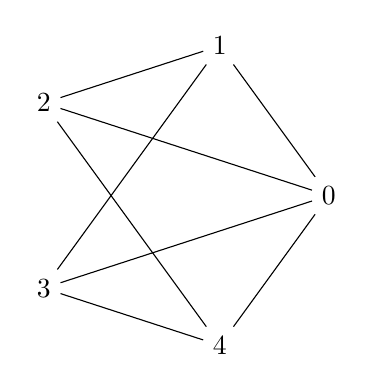
\begin{tikzpicture}
      \draw
        (0.0:2) node (0){0}
        (72.0:2) node (1){1}
        (144.0:2) node (2){2}
        (216.0:2) node (3){3}
        (288.0:2) node (4){4};
      \begin{scope}[-]
        \draw (0) to (1);
        \draw (0) to (2);
        \draw (0) to (3);
        \draw (0) to (4);
        \draw (1) to (2);
        \draw (1) to (3);
        \draw (2) to (4);
        \draw (3) to (4);
      \end{scope}
    \end{tikzpicture}
\end{figure}
\begin{itemize}
\item signature: 1111110011
\item g: Graph with 5 nodes and 8 edges
\item order: 5
\item size: 8
\item max degree: 4
\item degrees: 3,3,3,3,4
\item is tree: 0
\item is bipartite: 0
\item has bridge: 0
\item is chordal: 0
\item is complete: 0
\item min cycle basis weight: 12
\item min cycle basis size: 4
\item diameter: 2
\item radius: 1
\item is eulerian: 0
\item is planar: 1
\item number of faces: 5
\item is regular: 0
\item p3: 6
\item p4: None
\item property hash: cb551c444d1e1633bc2a5f42b7f8f05216ee555cf9cfbda0f6cf794da73e3133
\end{itemize}
\newpage
